\documentclass{beamer}
\def\java{\texttt{Java}}
\def\mytoday{30 November 2016}
\def\mpause{\pause}
\usepackage{pgfpages}\def\mpause{\pause}
%\usepackage{pgfpages}\pgfpagesuselayout{8 on 1}[a4paper,border shrink=1mm, landscape]\def\mpause{}
\usepackage{url}
\usepackage{verbatim}
\usepackage{color}
\usepackage{listings}
\usepackage{code}
\usepackage{textcomp}
%\usepackage{epsfig}
\usepackage{graphicx}

%\usepackage{bm}
\usepackage{beamerthemesplit}
\defbeamertemplate*{footline}{infolines theme}{
\hspace*{2ex}    \insertframenumber{} / \inserttotalframenumber\hspace*{2ex} 
\copyright Manfred Kerber
%   \insertpagenumber{} / \insertpresentationendpage \hspace*{2ex}
  \vskip1ex}

\def\mcolor#1#2{\rule{0ex}{0ex}\color{#1}#2\color{black}{}}
\usetheme{Copenhagen}
%\setbeamercolor{title}{fg=red!80!black,bg=red!20!white}
\makeatletter % code block to allow custom labels to be cross-ref'ed; see comp.text.tex "customized display labels cross-ref'd"
\begin{document}

\title{MSc/ICY Software Workshop\\
Graphical User Interfaces}

\author[Manfred~Kerber]{\begin{tabular}{ll}
\mcolor{blue}{Manfred Kerber} &   {\tt www.cs.bham.ac.uk/\~{}mmk}
\end{tabular}\\[1ex]
(Slides mainly taken from Jon Rowe's corresponding lecture in Software Workshop 1, 2015, with some modifications)
}

\date{\mytoday}

\begin{frame}
\titlepage
\end{frame}

\begin{frame}[fragile]
\frametitle{Model -‐ View -- Control}
\begin{itemize}
\item When creating a graphical user interface (GUI) for a program, we
  try to keep the \mcolor{blue}{program functionality (model)} \mcolor{red}{separate from} the
  \mcolor{blue}{display elements (views)} and \mcolor{blue}{interaction elements (controls)}.

\item We use the Observer -- Observable pattern to do this -- it
  enables a clean separation that is easy to maintain.
\end{itemize}
\end{frame}

\begin{frame}
\frametitle{Model -‐ View -- Controller (Cont'd)}
\begin{center}
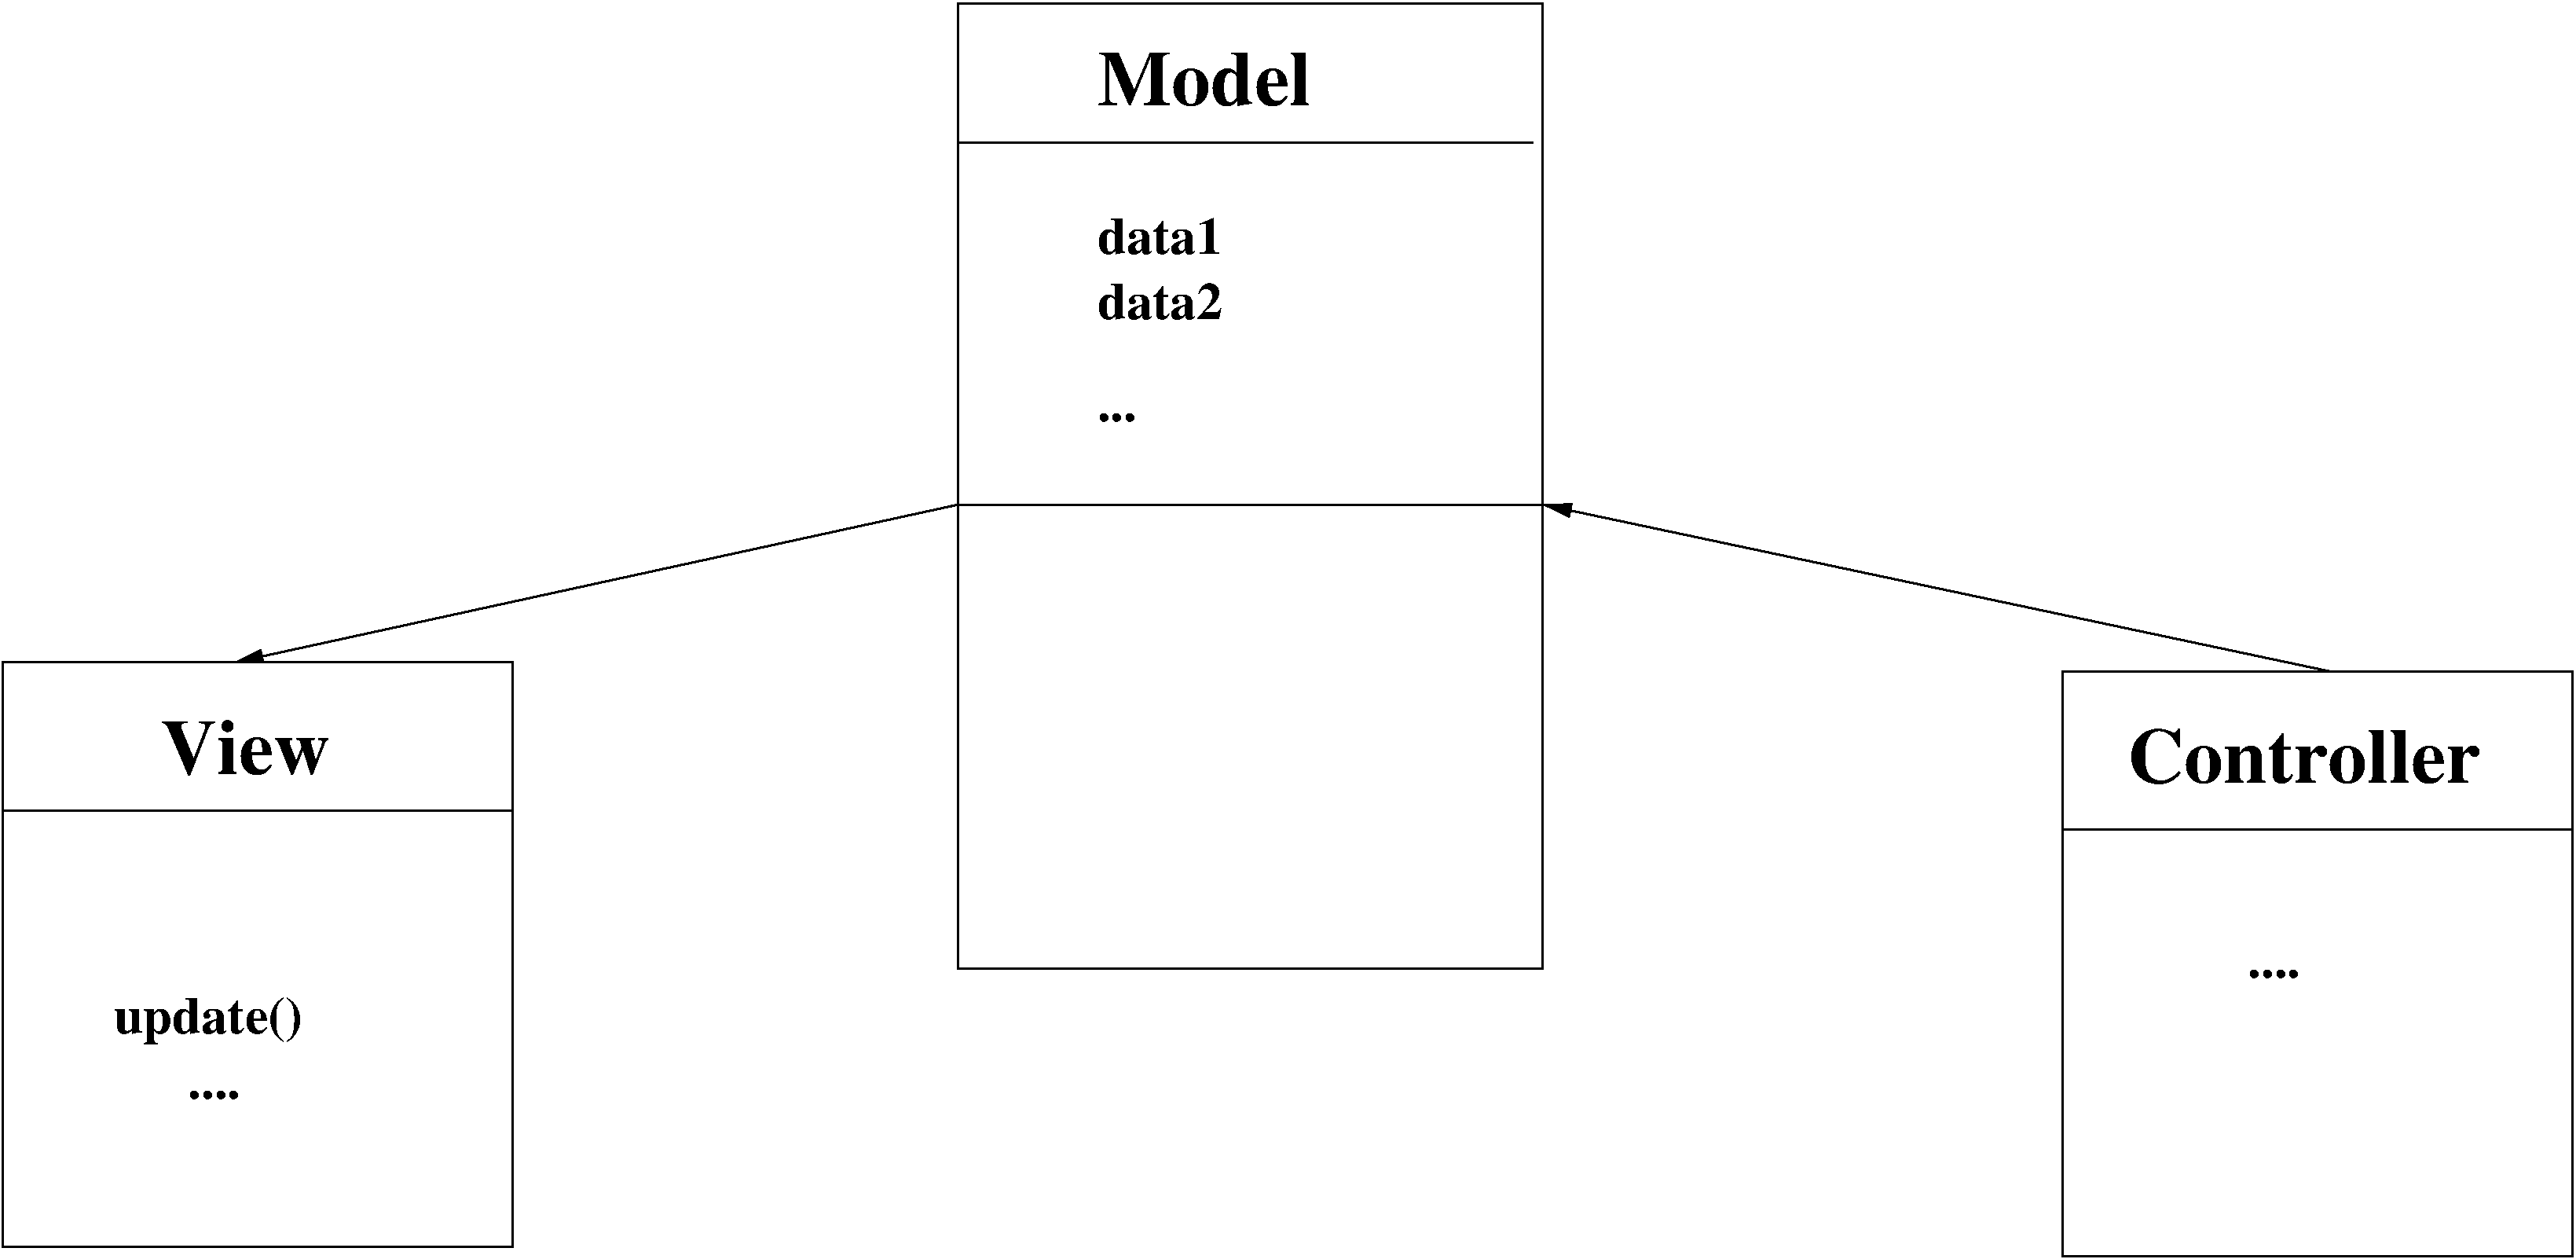
\includegraphics[width=0.9\textwidth]{./model-view-control.pdf}

Taken from Walter Savitch, Absolute Java, p.1006
\end{center}
\end{frame}

\begin{frame}
\frametitle{Observer -- Observable}
\begin{itemize}
\item We ``wrap'' the underlying program objects into a ``model''
  object.
\item The model object is from a class that extends \texttt{Observable}.
\item This means that it can have observers (using \texttt{addObserver}).
\item When a change occurs, the observers are notified:\\
\texttt{setChanged();}\\
\texttt{notifyObservers();}
\end{itemize}
\end{frame}

\begin{frame}
  \frametitle{Views are observers}
\begin{itemize}
\item We make any view class extend the type of view it is (e.g.
  \texttt{JLabel}), and implement the \texttt{Observer} interface.

\item This means it must provide a method:\\
  \texttt{public void update(Observable obs, Object obj)}
	  
\item This is the method that is run when \texttt{notifyObservers()} is
  called.
\end{itemize}
\end{frame}

\begin{frame}
  \frametitle{Controls and Listeners}
\begin{itemize}
\item Elements that the user can interact with are called controls.
\item Often you can use the built-in control class directly (e.g.
  \texttt{JSlider}), but you can create your own class for them if you
  want to add extra functionality.
\begin{center}
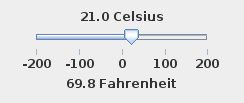
\includegraphics[width=0.4\textwidth]{./slider.png}
\end{center}
\item Each control needs a listener to handle the interactions.
\end{itemize}
\end{frame}

\begin{frame}
  \frametitle{Listeners and events}
\begin{itemize}
\item When the user interacts with a control, it generates an
  ``\texttt{event}'' object.
\item For example, moving the slider creates a \mcolor{blue}{\texttt{ChangeEvent}}
  object.
\item The compiler looks to see if there is a listener attached to the
  control that can handle the event.
\item If so, the appropriate method is run. 
\end{itemize}
\end{frame}

\begin{frame}
\frametitle{Implementing Listeners}
\begin{itemize}
\item Listeners are interfaces.
\item There are different listener interfaces for different kinds of
  control and event.
\item For example, to handle a \mcolor{blue}{\texttt{ChangeEvent}}, you need a \mcolor{blue}{\texttt{ChangeListener}}.
\item This requires you to provide the appropriate method:\\
\mcolor{blue}{\texttt{public void stateChanged(ChangeEvent e)}}
\end{itemize}
\end{frame}

\begin{frame}
\frametitle{The sequence of events}
\begin{itemize}
\item The user interacts with a control.
\item This generates an event.
\item The listener handles the event and runs its method.
\item This creates changes in the model.
\item The model's set methods call \mcolor{blue}{\texttt{notifyObservers}}.
\item All the views that are observing the model run their update
  method.
\item This causes them to re-draw themselves appropriately.  
\end{itemize}
\end{frame}


\begin{frame}
\frametitle{Recipe for writing a GUI}
\begin{itemize}
\item Create \mcolor{blue}{model} class (wraps underlying program objects, abstracts the program functionality).
\item Create \mcolor{blue}{view} classes, one for each view
\item Create \mcolor{blue}{control} classes, if needed.
\item Create \mcolor{blue}{listener} classes, one for each event.
\item Create \mcolor{blue}{component} class to house everything.
\item Create \mcolor{blue}{GUI} class with main method. 
\end{itemize}
\end{frame}


\begin{frame}
  \frametitle{Create model class}
\begin{itemize}
\item Your model class should have as data fields all the program
  objects you need.
\item It should \mcolor{blue}{extend \texttt{Observable}}.
\item Provide wrapper methods for the get methods you need for your
  GUI.
\item Provide wrapper set methods.
\item The set methods should call\\
\mcolor{blue}{\texttt{setChanged();}}\\
\mcolor{blue}{\texttt{notifyObservers();}}
\end{itemize}
\end{frame}


\begin{frame}
\frametitle{Create view classes}
\begin{itemize}
\item For each disjoint view, you need a separate class.
\item The class should extend the type of component you want it to be
  (e.g.\ \texttt{JLabel}).
\item It should implement \texttt{Observer}.
\item \mcolor{blue}{You have to provide the update method, which says how to
  re‐draw itself if it is told the model has changed.}
\end{itemize}
\end{frame}

\begin{frame}
\frametitle{Create control classes}
\begin{itemize}
\item For each distinct control, you need to decide whether it needs
  its own class, or if you can use the built in class directly (e.g.
  \texttt{JSlider}).
\item \mcolor{blue}{You only need a new class (which extends the component class) if
  you are adding functionality.}
\item For example, this might happen if the control is also a view.
\end{itemize}
\end{frame}

\begin{frame}
\frametitle{Create listener classes}
\begin{itemize}
\item \mcolor{blue}{For each different control and different event
    type, you need a listener.}
\item You have to look up what kind of listener goes with what kind of
  control and event.
\item The class should implement that listener.
\item It is helpful for it to have the model and the control as data
  fields.
\item You need to implement the appropriate method to handle the
  event.  Typically it changes the model.
\end{itemize}
\end{frame}

\begin{frame}
  \frametitle{Create component class }
\begin{itemize}
\item \mcolor{blue}{Typically we use \texttt{JPanel}, rather than \texttt{JComponent}.}
\item This allows several components to be displayed at once.
\item You need the constructor, to create all the parts and plug them
  together.
\item If you have any extra graphics, you might need to override
  \texttt{paintComponent}.  
\end{itemize}
\end{frame}

\begin{frame}
  \frametitle{Component constructor recipe}
\begin{itemize}
\item Should take program objects as arguments.  
\item Call \texttt{super();}
\item Create \mcolor{blue}{model objects}.
\item Create \mcolor{blue}{view objects}.
\item \mcolor{blue}{Make views observe the model.}
\item Create \mcolor{blue}{control} objects.
\item Create \mcolor{blue}{listener} objects.
\item \mcolor{blue}{Make listeners listen to controls.}
\item \mcolor{blue}{Put views and controls on to panel.}
\end{itemize}
\end{frame}

\begin{frame}
  \frametitle{Create GUI}
\begin{itemize}
\item In this class you will have your main method.
\item This should create \mcolor{blue}{program objects}.
\item Then create the \mcolor{blue}{component} (JPanel).
\item Then create the \mcolor{blue}{frame}.
\item \mcolor{blue}{Put the component on the frame.}
\item Make everything \mcolor{blue}{visible}.
\end{itemize}
\end{frame}

\begin{frame}
  \frametitle{Create GUI (Cont'd)}
\begin{center}
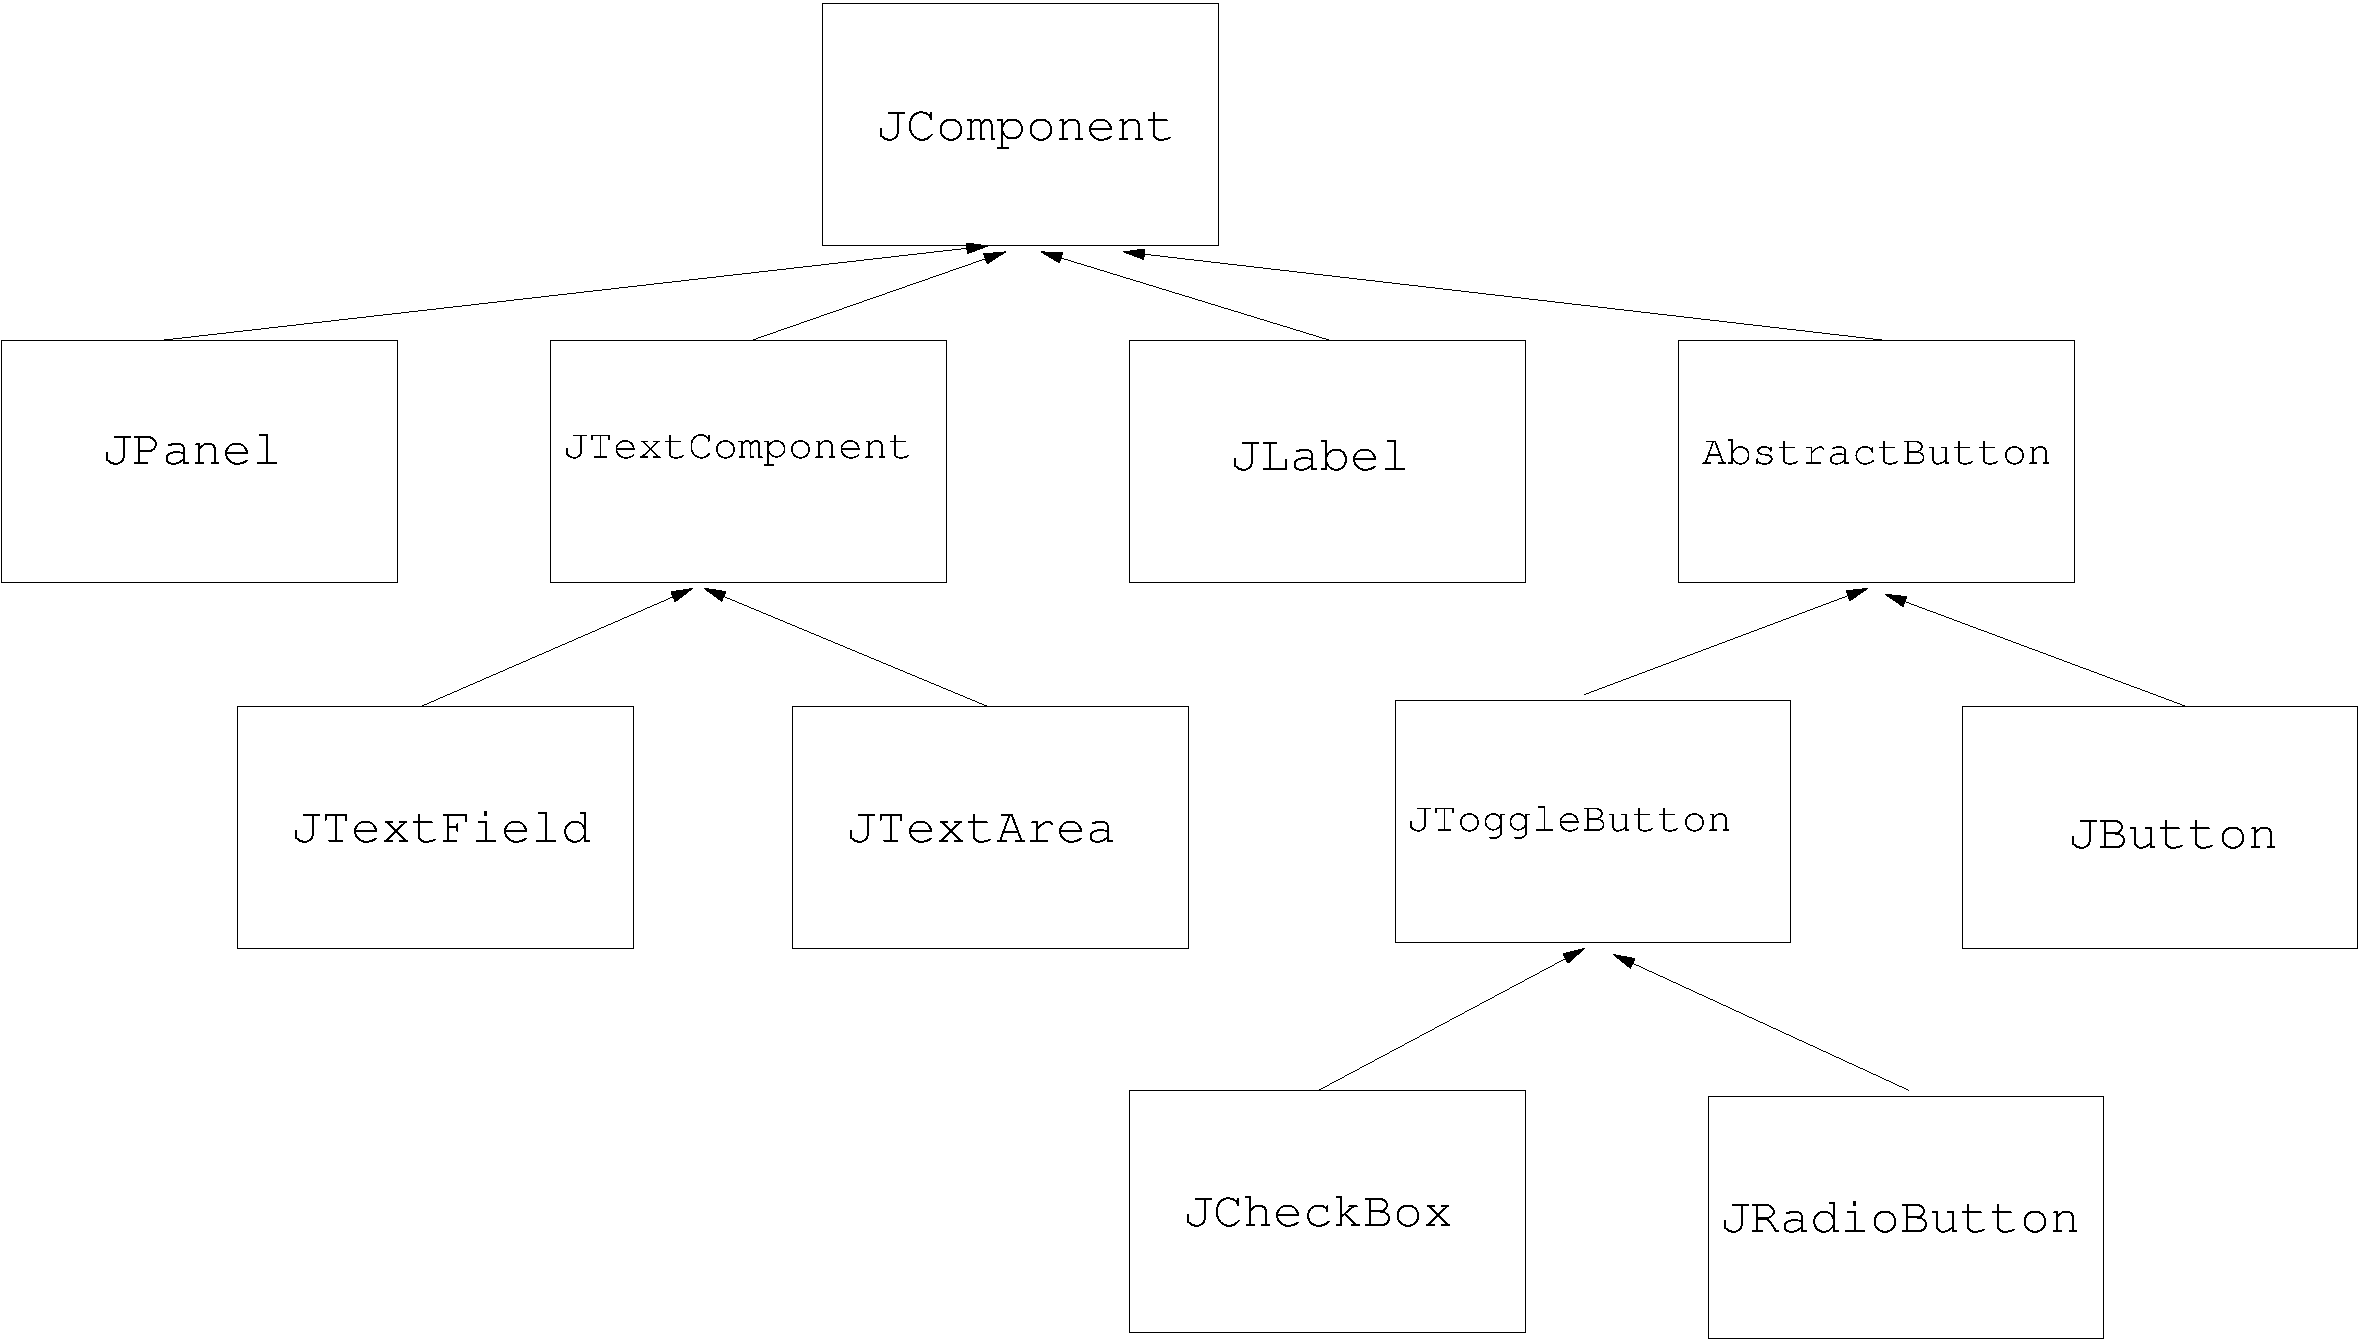
\includegraphics[width=1\textwidth]{./swingHierarchy.pdf}
\end{center}

A Part of the Hierarch of Swing User-Interface Components (taken from Horstmann ``Big Java'' 4th Edition, p. 721).
\end{frame}

\begin{frame}
  \frametitle{Getting organized}
\begin{itemize}
\item The key to writing a good GUI is to get organized.
\item \mcolor{blue}{Sketch how you want it to look on paper.}
\item Then \mcolor{blue}{make a list of all the views, controls and
    listeners} you will need.
\item Write them one by one, working your way through the list.
\item Do not forget to plug everything together!  
\end{itemize}
\end{frame}

\begin{frame}
  \frametitle{Note on Observer pattern}
\begin{itemize}
\item \mcolor{blue}{The Observer pattern allows a very clean
    separation of Model -- View -- Control.}
\item However, it is not necessarily very efficient (why?).
\item \mcolor{blue}{Developers often do not use it -- instead they
    make their control listeners directly manipulate views as well as
    the model.}
\item This is more efficient -- but potentially messier to write and
  maintain.
\end{itemize}
\end{frame}



\end{document}


%%% Local Variables: 
%%% mode: latex
%%% TeX-master: "slides"Superclasses
%%% End: 

